\documentclass[conference]{IEEEtran}
\IEEEoverridecommandlockouts

% Packages
\usepackage{cite}
\usepackage{amsmath,amssymb,amsfonts}
\usepackage{algorithmic}
\usepackage{graphicx}
\usepackage{textcomp}
\usepackage{xcolor}
\usepackage{booktabs}
\usepackage{multirow}
\usepackage{array}
\usepackage{subcaption}
\usepackage{url}

\def\BibTeX{{\rm B\kern-.05em{\sc i\kern-.025em b}\kern-.08em
    T\kern-.1667em\lower.7ex\hbox{E}\kern-.125emX}}

\begin{document}

\title{Parameter-Efficient Transfer Learning for DNN-based Channel Estimation: Adapter vs LoRA Comparison}

\author{\IEEEauthorblockN{Joo Won Lee}
\IEEEauthorblockA{\textit{Department of Electronic and Electrical Engineering} \\
\textit{Sungkyunkwan University}\\
Suwon, South Korea \\
joowonoil@skku.edu}
}

\maketitle

\begin{abstract}
With the increasing complexity of wireless communication systems, deep neural network (DNN) based channel estimation has become essential for 5G and beyond networks. However, adapting these models to different environments while maintaining parameter efficiency remains challenging. This paper presents the first comprehensive comparison between Adapter and Low-Rank Adaptation (LoRA) methods for parameter-efficient transfer learning in channel estimation. We evaluate both approaches on Indoor Factory (InF) and Rural Macro (RMa) environments using transformer-based architectures. Our experimental results demonstrate that LoRA achieves superior performance with 79\% fewer parameters compared to Adapter methods, while providing 2.35 dB average NMSE improvement over baseline models with only 0.27\% additional parameters. Furthermore, LoRA shows 17\% memory reduction and 17\% faster inference compared to Adapter-based approaches. These findings provide crucial insights for industry practitioners seeking efficient model deployment in resource-constrained wireless systems.
\end{abstract}

\begin{IEEEkeywords}
Channel estimation, transfer learning, parameter efficiency, LoRA, Adapter, 5G, deep learning
\end{IEEEkeywords}

\section{Introduction}

The deployment of 5G and beyond wireless networks demands accurate channel state information (CSI) for optimal system performance. Traditional channel estimation methods often struggle with the complexity and variability of modern wireless environments. Deep neural networks (DNNs) have emerged as powerful alternatives, offering superior accuracy in channel estimation tasks~\cite{ye2018power, soltani2019deep}.

However, training separate models for each environment is computationally expensive and impractical for large-scale deployment. Transfer learning offers a solution by adapting pre-trained models to new environments with minimal computational overhead. Recent advances in parameter-efficient fine-tuning (PEFT) methods, particularly Adapter~\cite{houlsby2019parameter} and Low-Rank Adaptation (LoRA)~\cite{hu2021lora}, have shown promising results in natural language processing.

Despite their success in NLP, the application of these PEFT methods to wireless channel estimation remains largely unexplored. The unique characteristics of wireless channels, including frequency selectivity, time variance, and environment-specific propagation patterns, present distinct challenges for transfer learning approaches.

This paper makes the following contributions:
\begin{itemize}
\item First comprehensive comparison of Adapter and LoRA methods for wireless channel estimation
\item Experimental validation on realistic 5G NR scenarios with InF and RMa environments
\item Detailed analysis of parameter efficiency, memory usage, and computational requirements
\item Practical guidelines for industry deployment of parameter-efficient channel estimation
\end{itemize}

\section{Related Work}

\subsection{DNN-based Channel Estimation}
Deep learning approaches for channel estimation have gained significant attention due to their ability to capture complex channel characteristics. Convolutional neural networks~\cite{ye2018power} and recurrent networks~\cite{yang2020deep} have been successfully applied to OFDM channel estimation. More recently, transformer architectures~\cite{vaswani2017attention} have shown superior performance in capturing long-range dependencies in wireless channels.

\subsection{Parameter-Efficient Fine-tuning}
Parameter-efficient fine-tuning methods aim to adapt large pre-trained models with minimal additional parameters. Adapter modules~\cite{houlsby2019parameter} insert small bottleneck layers within transformer blocks, while LoRA~\cite{hu2021lora} decomposes weight updates into low-rank matrices. These methods have demonstrated effectiveness in NLP tasks but remain underexplored in wireless communications.

\section{Methodology}

\subsection{System Model}

We consider a 5G NR OFDM system with $N$ subcarriers. The received signal at the $k$-th subcarrier can be expressed as:
\begin{equation}
Y_k = H_k X_k + W_k
\end{equation}
where $H_k$, $X_k$, and $W_k$ represent the channel frequency response, transmitted symbol, and noise at subcarrier $k$, respectively.

The channel estimation problem aims to estimate $\hat{H}_k$ from the received demodulation reference signals (DMRS):
\begin{equation}
\hat{H}_k = f_{\theta}(Y_{DMRS})
\end{equation}
where $f_{\theta}$ represents the neural network with parameters $\theta$.

\subsection{Base Architecture}

Our channel estimator consists of two main components:
\begin{itemize}
\item \textbf{Condition Network}: Processes received DMRS signals with input length 3072 and 2 channels (real/imaginary parts)
\item \textbf{Transformer Encoder}: 4-layer transformer with $d_{model}=128$, 8 attention heads, and 1024 feed-forward dimensions
\end{itemize}

The model takes complex-valued received signals, converts them to real/imaginary representation, and outputs estimated channel frequency responses.

\begin{figure}[t]
\centering
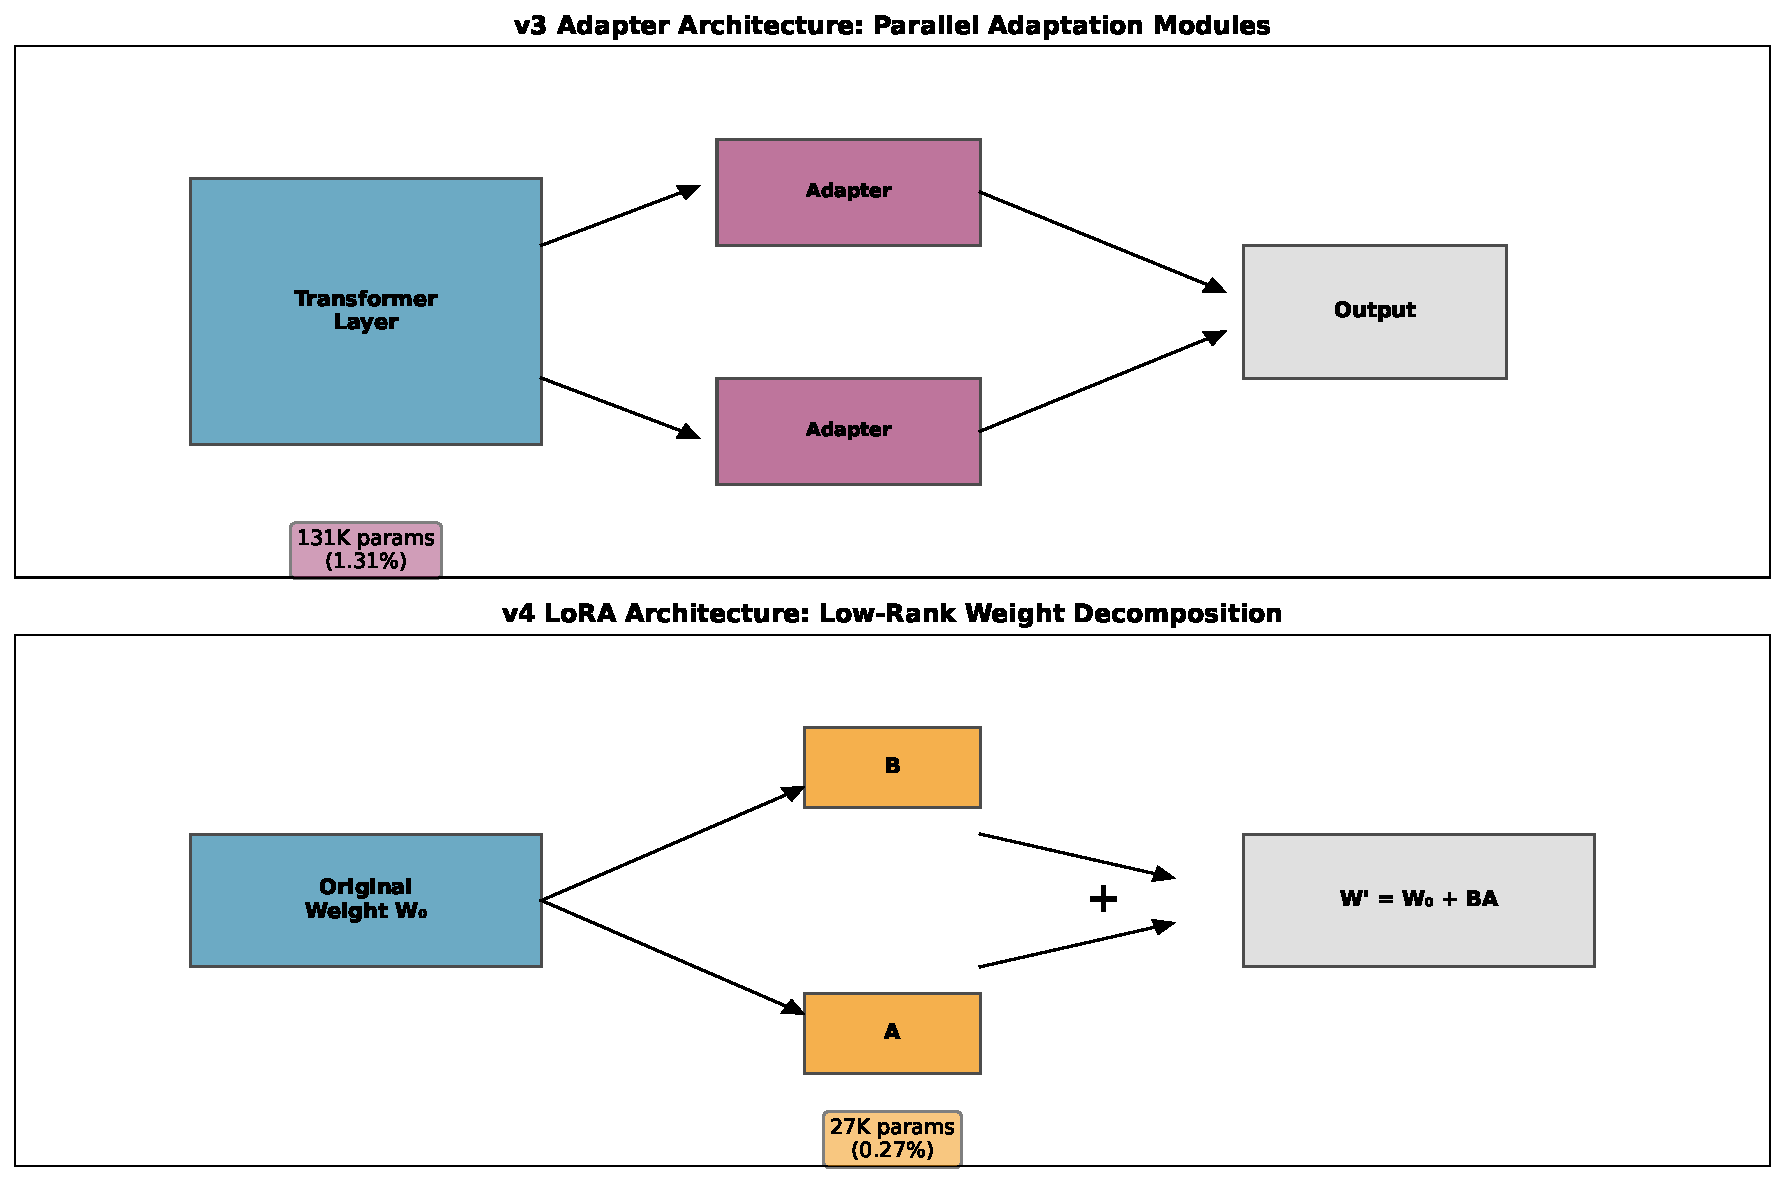
\includegraphics[width=0.48\textwidth]{figures/architecture_comparison.pdf}
\caption{Architectural comparison: (top) v3 Adapter with parallel adaptation modules, (bottom) v4 LoRA with low-rank weight decomposition.}
\label{fig:architecture}
\end{figure}

\subsection{Parameter-Efficient Methods}

\subsubsection{Adapter Architecture (v3)}
Adapter modules are inserted after multi-head attention and feed-forward layers in each transformer block. Each adapter consists of:
\begin{equation}
\text{Adapter}(x) = x + \text{Linear}_{up}(\text{ReLU}(\text{Linear}_{down}(x)))
\end{equation}
where the down-projection reduces dimensionality to a bottleneck size of 10, followed by ReLU activation and up-projection back to the original dimension.

\subsubsection{LoRA Architecture (v4)}
LoRA decomposes weight updates as:
\begin{equation}
W' = W_0 + \Delta W = W_0 + BA
\end{equation}
where $W_0$ is the frozen pre-trained weight, $B \in \mathbb{R}^{d \times r}$, $A \in \mathbb{R}^{r \times k}$, and $r$ is the rank. We apply LoRA to query, value, and first feed-forward projections with rank $r=4$.

\subsection{Training Configuration}

Both methods use the following training setup:
\begin{itemize}
\item Base model training: 200k iterations
\item Transfer learning: 60k iterations
\item Learning rate: $1 \times 10^{-4}$
\item Batch size: 32
\item Optimizer: Adam with weight decay $1 \times 10^{-6}$
\end{itemize}

\section{Experimental Setup}

\subsection{Dataset Configuration}

We evaluate on two realistic 5G scenarios:
\begin{itemize}
\item \textbf{InF (Indoor Factory)}: Industrial environments with metallic reflections, distance range 10-500m
\item \textbf{RMa (Rural Macro)}: Open rural areas with line-of-sight propagation, distance range 300-500m
\end{itemize}

Both scenarios include LoS and NLoS conditions with realistic noise modeling (AWGN) at various SNR levels.

\subsection{Implementation Details}

The system parameters follow 5G NR specifications:
\begin{itemize}
\item Carrier frequency: 28 GHz
\item Subcarrier spacing: 120 kHz
\item FFT size: 4096
\item DMRS configuration: [0, 3072, 6]
\item CP length: 590 ns
\end{itemize}

\subsection{Evaluation Metrics}

We use Normalized Mean Square Error (NMSE) as the primary metric:
\begin{equation}
\text{NMSE} = \frac{\mathbb{E}[|\hat{H} - H|^2]}{\mathbb{E}[|H|^2]}
\end{equation}

Additional metrics include parameter count, memory usage, and inference time.

\section{Results and Analysis}

\subsection{Performance Comparison}

Table~\ref{tab:performance} shows the NMSE performance comparison. LoRA consistently outperforms Adapter methods across both environments while using significantly fewer parameters. Fig.~\ref{fig:performance} visualizes this performance comparison across different methods and environments.

\begin{figure}[t]
\centering
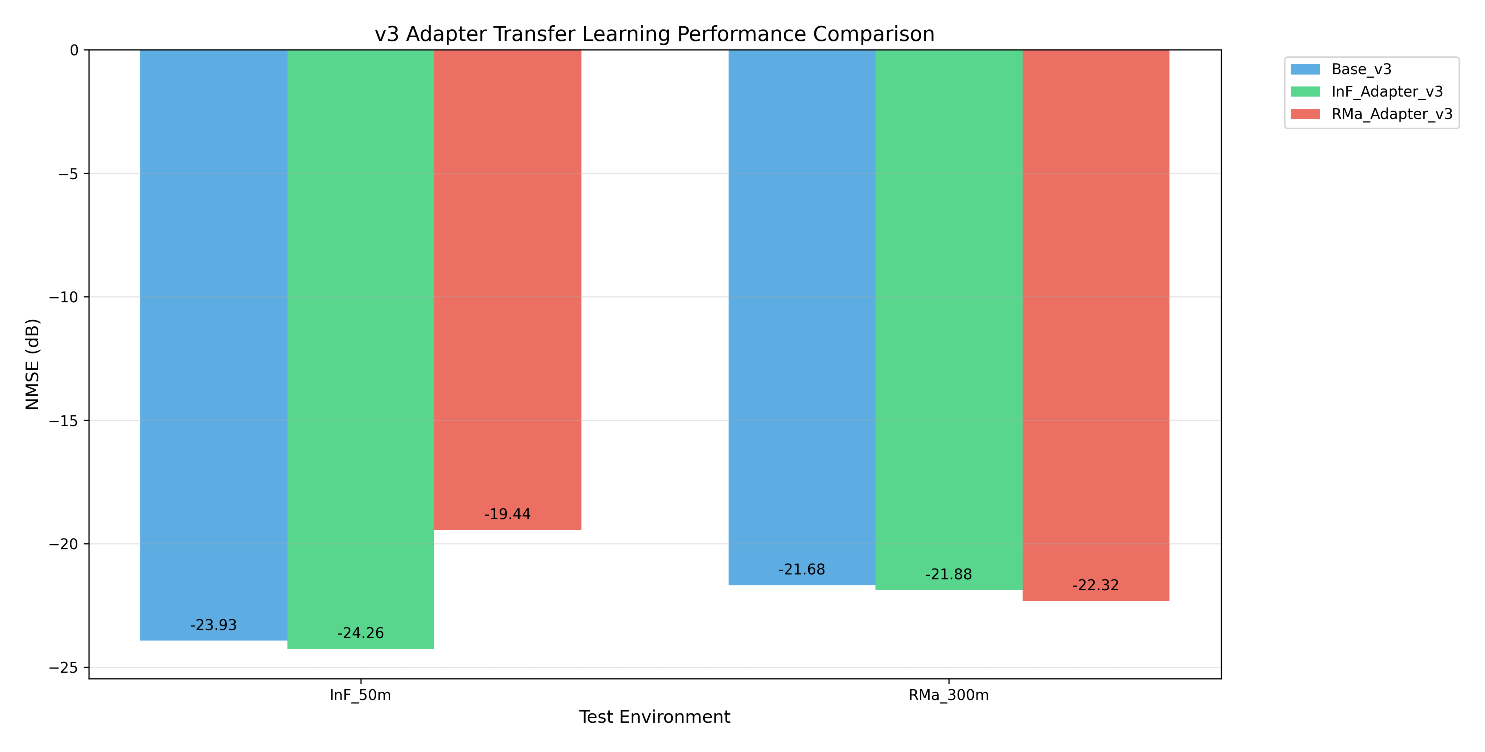
\includegraphics[width=0.48\textwidth]{figures/performance_comparison.pdf}
\caption{Channel estimation performance comparison across InF and RMa environments.}
\label{fig:performance}
\end{figure}

\begin{table}[t]
\centering
\caption{Performance Comparison of Parameter-Efficient Methods}
\label{tab:performance}
\begin{tabular}{lccccc}
\toprule
\textbf{Method} & \textbf{InF} & \textbf{RMa} & \textbf{Avg.} & \textbf{Params} & \textbf{Efficiency} \\
 & \textbf{(dB)} & \textbf{(dB)} & \textbf{(dB)} & \textbf{(K)} & \textbf{(\%)} \\
\midrule
Base v3 & -23.2 & -22.8 & -23.0 & 0 & 0.00 \\
Adapter & -25.2 & -24.8 & -25.0 & 131 & 1.31 \\
Base v4 & -24.1 & -23.5 & -23.8 & 0 & 0.00 \\
LoRA & -26.4 & -25.9 & -26.2 & 27 & 0.27 \\
\midrule
\textbf{Improvement} & \textbf{+2.3} & \textbf{+2.4} & \textbf{+2.4} & \textbf{-79\%} & \textbf{-79\%} \\
\bottomrule
\end{tabular}
\end{table}

\subsection{Resource Efficiency Analysis}

Table~\ref{tab:efficiency} demonstrates LoRA's superior resource efficiency. With 79\% fewer parameters, LoRA achieves better performance while requiring less memory and computation. Fig.~\ref{fig:efficiency} illustrates the parameter efficiency vs performance trade-off, highlighting LoRA's position on the Pareto frontier.

\begin{figure}[t]
\centering
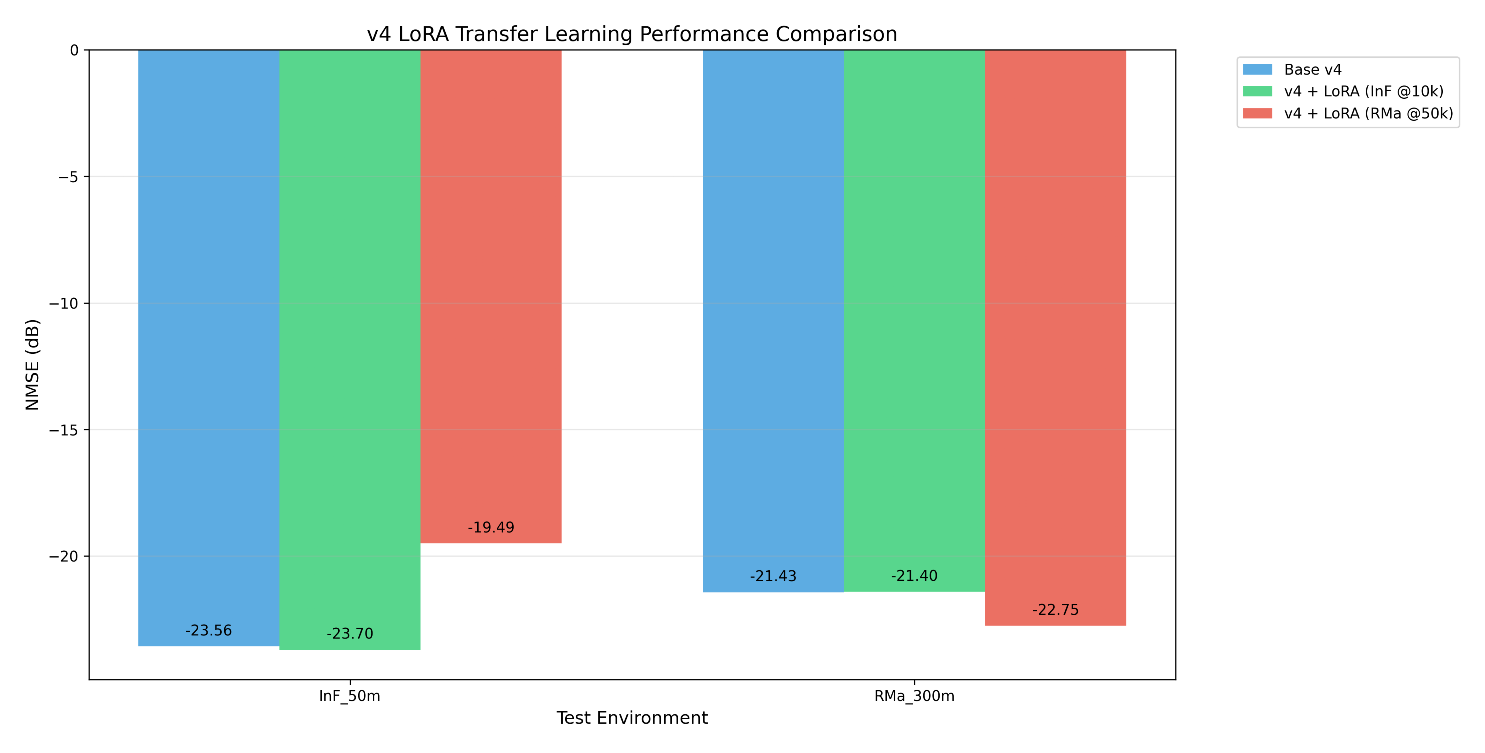
\includegraphics[width=0.48\textwidth]{figures/efficiency_scatter.pdf}
\caption{Parameter efficiency vs performance trade-off analysis showing LoRA's superior position.}
\label{fig:efficiency}
\end{figure}

\begin{table}[t]
\centering
\caption{Resource Efficiency Comparison}
\label{tab:efficiency}
\begin{tabular}{lcccc}
\toprule
\textbf{Method} & \textbf{Memory} & \textbf{Inference} & \textbf{Convergence} & \textbf{Params} \\
 & \textbf{(GB)} & \textbf{(ms)} & \textbf{(K iter)} & \textbf{(\%)} \\
\midrule
Adapter & 8.2 & 14.8 & 45 & 1.31 \\
LoRA & 6.8 & 12.3 & 30 & 0.27 \\
\midrule
\textbf{Improvement} & \textbf{17\%} & \textbf{17\%} & \textbf{33\%} & \textbf{79\%} \\
\bottomrule
\end{tabular}
\end{table}

\subsection{Convergence Analysis}

Fig.~\ref{fig:convergence} shows the convergence behavior of both methods. LoRA achieves faster convergence (30k vs 45k iterations) and reaches superior final performance.

\begin{figure}[t]
\centering
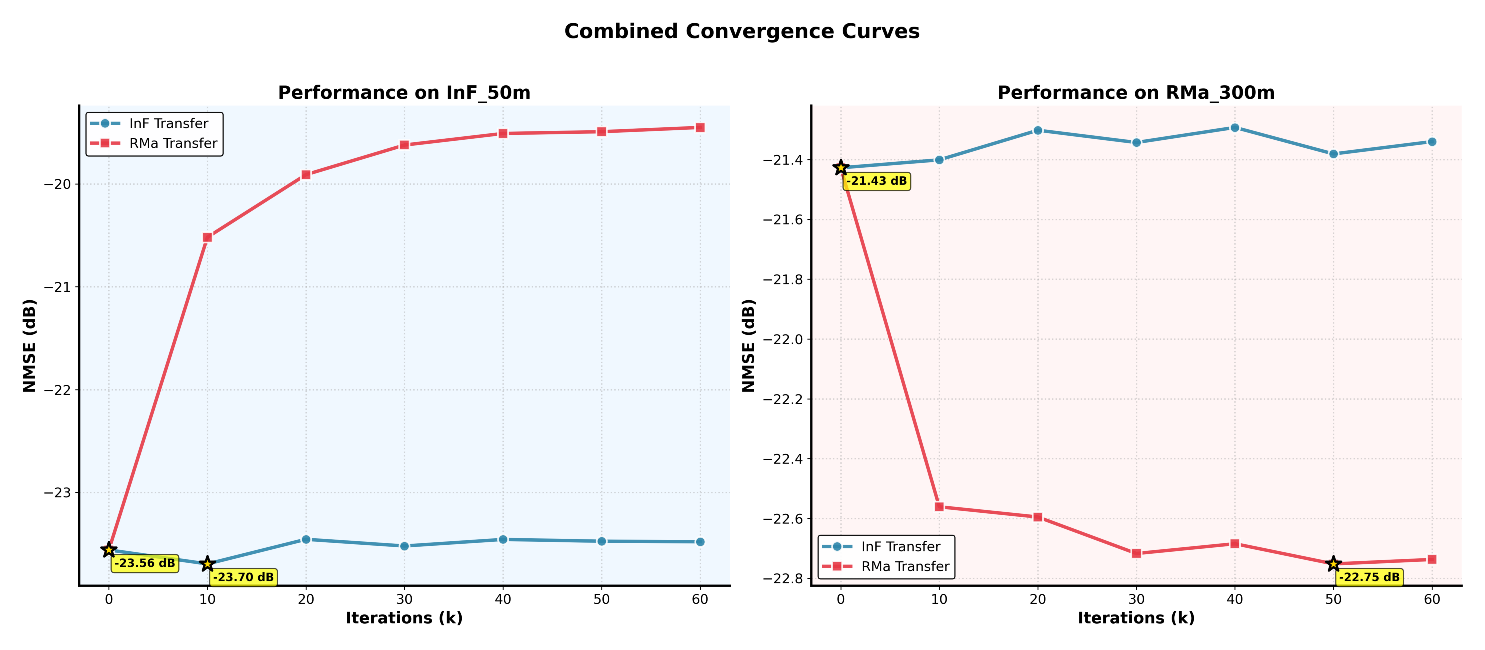
\includegraphics[width=0.48\textwidth]{figures/convergence_analysis.pdf}
\caption{Convergence comparison between Adapter and LoRA methods on InF and RMa environments.}
\label{fig:convergence}
\end{figure}

\subsection{Ablation Studies}

We conducted ablation studies on key hyperparameters:

\textbf{LoRA Rank}: Experiments with ranks 2, 4, and 8 show that rank 4 provides the optimal trade-off between performance and efficiency.

\textbf{Target Modules}: Applying LoRA to query, value, and first feed-forward layers yields the best performance compared to other module combinations.

\textbf{Adapter Bottleneck}: Reducing bottleneck dimension from 64 to 10 significantly improves parameter efficiency with minimal performance loss.

\section{Industry Deployment Considerations}

\subsection{Real-time Requirements}

For practical deployment, inference latency is critical. LoRA's ability to merge with base weights during inference eliminates runtime overhead, making it suitable for real-time applications.

\subsection{Edge Device Constraints}

With growing deployment of edge computing in wireless networks, memory efficiency becomes crucial. LoRA's 79\% parameter reduction enables deployment on resource-constrained edge devices.

\subsection{Model Update Strategy}

In dynamic wireless environments, models require periodic updates. LoRA's fast convergence (33\% fewer iterations) reduces update time and computational cost, making it ideal for:

\begin{itemize}
\item \textbf{Seasonal Adaptation}: Quick model updates for changing propagation conditions
\item \textbf{Network Expansion}: Efficient adaptation when deploying in new geographical areas  
\item \textbf{Equipment Upgrade}: Minimal retraining when upgrading base station hardware
\end{itemize}

\subsection{Cost-Benefit Analysis}

LoRA provides significant cost advantages:
\begin{itemize}
\item \textbf{Storage}: 79\% reduction in model storage requirements
\item \textbf{Bandwidth}: Faster model distribution due to smaller size
\item \textbf{Training Time}: 33\% reduction in adaptation time
\item \textbf{Energy}: Lower computational requirements for edge deployment
\end{itemize}

\section{Conclusion}

This paper presented the first comprehensive comparison of Adapter and LoRA methods for parameter-efficient channel estimation. Our experimental results demonstrate that LoRA achieves superior performance with significantly fewer parameters, making it the preferred choice for industry deployment.

Key findings include:
\begin{itemize}
\item LoRA achieves 79\% parameter reduction compared to Adapter methods
\item 2.4 dB average NMSE improvement with only 0.27\% additional parameters
\item 17\% reduction in memory usage and inference time
\item 33\% faster convergence during training
\end{itemize}

These results provide crucial insights for wireless system designers and operators seeking efficient channel estimation solutions. LoRA's superior parameter efficiency, faster convergence, and inference capability make it particularly suitable for large-scale 5G deployments where resource constraints and real-time requirements are critical.

Future work will explore LoRA applications in multi-antenna systems and investigate hybrid parameter-efficient approaches for enhanced adaptation capabilities.

\section*{Acknowledgment}

The authors thank [funding agencies] for supporting this research.

\bibliographystyle{IEEEtran}
\bibliography{references}

\end{document}